% Chapter 7

\chapter{Solution choices}
\label{Chapter7}

After a long research period of time and direct experience on developing mobile application using the most known cross-platform (Xamarin) and hybrid (Cordova Phonegap) solution, we decided to go native. This decision was based mostly on the needs and the strict performance requirements related to the project. Thanks to a native implementation we can achieve better results in term of performance and in term of user experience of the application. At the choice of a native platform we picked  Android because it is the most spread mobile OS over mobile devices and it is open source even if mostly maintained by Google.

\section{Android Platform}
Android is a mobile operating system (OS) currently developed by Google, based on the Linux Kernel and designed primarily for touchscreen mobile devices such as smartphones and tablets. Android has the largest installed base of all operating systems of any kind. Android has been the best selling OS on tablets since 2013, and on smartphones it is dominant by any metric.\cite{ref18}
\begin{figure}[ht!]
	\centering
	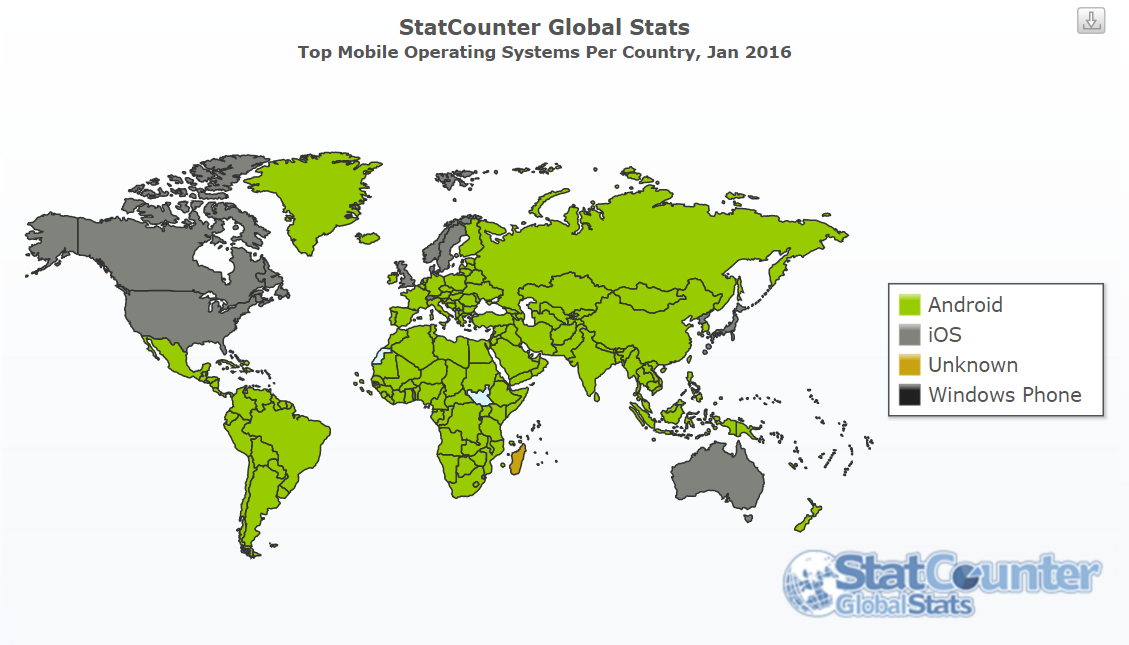
\includegraphics[width=120mm]{figures/ch7/1.png}
	\caption{Top Mobile Operating Systems Per Country, Jan 2016. Statcounter.com}
	\label{fig7.1}
\end{figure}
We have chosen to develop ECG-ira firstly on this platform because of it is widely spread over the world and its nature of being from an open source software made it stable and widely supported. The Android OS programming language is Java which is one of the most known and used OOP language for application and web development.

\section{Why native?}
The advantages of cross-platform (and hybrid) solution is mostly connected to code maintenance and to faster development, because most of the written codes stands for all the supported OS at building phase. Business logic and data structure can be easily share among the many OS for example by using Xamarin we can write unique code using C\# (c-sharp) and abstract the business logic, the web services and the database management independently from the specific platform we want to target.  Most of the time it is just a matter of working on different user interface, one for any supported OS. All of this look awesome and it is, but when it comes to performance metrics, custom interfaces and user experience, here we meet its weaknesses and limitations. ECG-ira main goal is to build up an usable and stable mobile medical application and to fulfill it we needed to exploit the native platform in order to achieve the best performance and the best user experience. As Android is the most spread mobile OS over smartphones and tablets it results in an obvious pick.\\
We believe native may not be the best pick for any kind of application. The choices has to be done according to the project requirements and goals. Pitfall for going native is the long development time and a deep (if not full) knowledge of that specific platform.

\section{Android concurrency exploitation}
As we have seen previously, a considerable computational effort is required to the app, especially during record acquisition. For this reason, the only way in order to guarantee a reasonable performance was to exploit the concurrency mechanisms available in the chosen platform. This decision will obviously increase the complexity of the execution: analyzing the execution of a single-threaded application is relatively simple because the order of execution is known. In multi-threaded applications, it is a lot more difficult to analyze how the program is executed and in which order the code is processed.\\
In the following paragraphs we will start from the basic mechanisms provided by Java language, and we will then analyse the ones, given available by the Android OS, that we have chosen to use in our application.

\subsection{Thread Overview}
Software programming is all about instructing the hardware to perform an action. The instructions are defined by the application code that the CPU processes in an ordered sequence, which is the high-level definition of a thread. From an application perspective, a thread is execution along a code path of Java statements that are performed sequentially. A code path that is sequentially executed on a thread is referred to as a task, a unit of work that coherently executes on one thread. A thread can either execute one or multiple tasks in sequence.

\subsubsection{Thread execution}
A thread in Java machine is represented by java.lang.Thread. It is the most basic execution environment in Android that executes tasks when it starts and terminates when the task is finished or there are no more tasks to execute; the alive time of the thread is determined by the length of the task. Thread supports execution of tasks that are implementations of the java.lang.Runnable interface. An implementation defines the task in the run method:
\begin{lstlisting}
	private class MyTask implements Runnable {
		public void run() {
			int i = 0; // Stored on the thread local stack.
		}
	}
\end{lstlisting}
All the local variables in the method calls from within a run() method—direct or indirect—will be stored on the local memory stack of the thread. The task’s execution is started by instantiating and starting a Thread:
\begin{lstlisting}
	Thread myThread = new Thread(new MyTask());
	myThread.start();
\end{lstlisting}
On the operating system level, the thread has both an instruction and a stack pointer. The instruction pointer references the next instruction to be processed, and the stack pointer references a private memory area—not available to other threads—where thread-local data is stored. Thread local data is typically variable literals that are defined in the Java methods of the application.\\
A CPU can process instructions from one thread at a time, but a system normally has multiple threads that require processing at the same time, such as a system with multiple simultaneously running applications. For the user to perceive that applications can run in parallel, the CPU has to share its processing time between the application threads. The sharing of a CPU’s processing time is handled by a scheduler. That determines what thread the CPU should process and for how long. The scheduling strategy can be implemented in various ways, but it is mainly based on the thread priority: a high-priority thread gets the CPU allocation before a low-priority thread and receive more execution time with respect to low-priority threads.\\
The execution of two concurrent threads can be done in java just declaring two Thread objects and then starting them by calling the method Thread .start():
\begin{lstlisting}
	Thread T1 = new Thread(new MyTask());
	T1.start();
\end{lstlisting}

\subsection{Threads in Android}
In Android there are basically three thread types:
\begin{itemize}
	\item \textbf{UI thread} (or main thread): it is started on application start and stays alive during the lifetime of the application process. The UI thread is the main thread of the application, used for executing Android components and updating the UI elements on the screen. If the platform detects that UI updates are attempted from any other thread, it will promptly notify the application by throwing a CalledFromWrongThreadException. This harsh platform behaviour is required because the Android UI Toolkit is not thread safe, so the runtime allows access to the UI elements from one thread only.
	\item \textbf{Binder threads}: they are used for communicating between threads in different processes. Each process maintains a set of threads, called a thread pool, that is never terminated or recreated, but can run tasks at the request of another thread in the process. These threads handle incoming requests from other processes, including system services, intents, content providers, and services.
	\item \textbf{Background threads}: All the threads that an application explicitly creates are background threads. This means that they have no predefined purpose, but are empty execution environments waiting to execute any task. The background threads are descendants of the UI thread, so they inherit the UI thread properties, such as its priority. By default, a newly created process does not contain any background threads. It is always up to the application itself to create them when needed.
\end{itemize}
The UI thread is the most important thread, but it gets no special scheduling advantage compared to the other threads—the scheduler is unaware of which thread is the UI thread. Instead, it is up to the application to not let the background threads interfere more than necessary with the UI thread.

\subsection{ Thread communication in Android}
In multithreaded applications, tasks can run in parallel and collaborate to produce a result. Hence, threads have to be able to communicate to enable true asynchronous processing.\\
The most common thread communication use case in Android is between the UI thread and worker threads. Hence, the Android platform defines its own message passing mechanism for communication between threads. The UI thread can offload long tasks by sending data messages to be processed on background threads. The message passing mechanism is a nonblocking consumer-producer pattern, where neither the producer thread nor the consumer thread will block during the message handoff.\\
The message handling mechanism in android is implemented with the following classes:
\begin{itemize}
	\item \textbf{android.os.Looper}: A message dispatcher associated with the one and only consumer thread.
	\item \textbf{android.os.Handler}: Consumer thread message processor and the interface for a producer thread to insert messages into the queue. A Looper can have many associated handlers, but they all insert messages into the same queue.
	\item \textbf{android.os.MessageQueue}: Unbounded linked list of messages to be processed on the consumer thread. Every Looper—and Thread—has at most one MessageQueue.
	\item \textbf{android.os.Message}: Message to be executed on the consumer thread.
\end{itemize}
	The mechanism is summarized in the figure \ref{fig7.2}.
\begin{figure}[ht!]
	\centering
	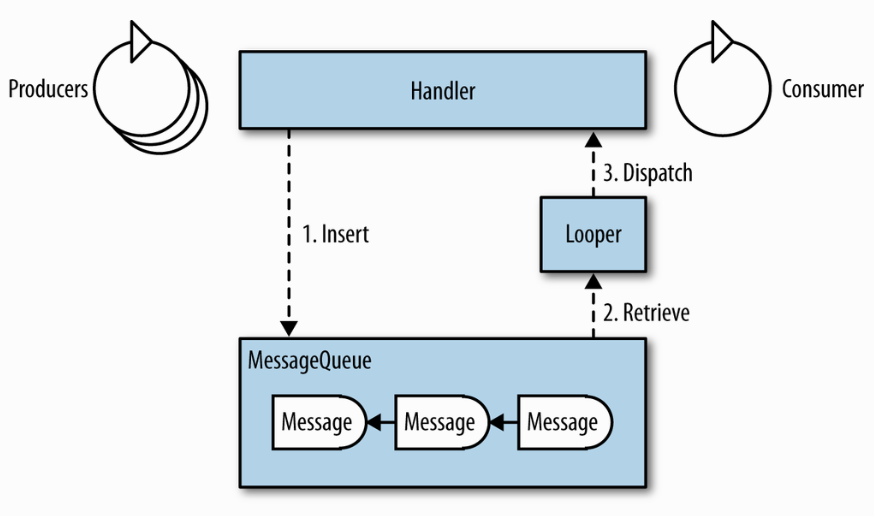
\includegraphics[width=120mm]{figures/ch7/2.png}
	\caption{Overview of the message-passing mechanism between multiple producer threads and one consumer thread.}
	\label{fig7.2}
\end{figure}
\begin{itemize}
	\item \textbf{Insert}: The producer thread inserts messages in the queue by using the Handler connected to the consumer thread.
	\item \textbf{Retrieve}: The Looper runs in the consumer thread and retrieves messages from the queue in a sequential order.
	\item \textbf{Dispatch}: The handlers are responsible for processing the messages on the consumer thread. A thread may have multiple Handler instances for processing messages; the Looper ensures that messages are dispatched to the correct Handler.
\end{itemize}

\subsection{HandlerThread}
Now we will describe a component that we have heavily exploited in our application, and as you will see in implementation details section, it represents the base of two main operations: the ECG signal drawing during both acquisition and record opening, and the ECG signal reading during record opening.\\
HandlerThread is a thread with a message queue that incorporates a Thread, a Looper, and a MessageQueue. It is constructed and started in the same way as a Thread. Once it is started, HandlerThread sets up queuing through a Looper and MessageQueue and then waits for incoming messages to process:
\begin{lstlisting}
	HandlerThread handlerThread = new HandlerThread("HandlerThread");
	handlerThread.start();
	
	mHandler = new Handler(handlerThread.getLooper()) {
		@Override
		public void handleMessage(Message msg) {
			super.handleMessage(msg);
			// Process messages here
		}
	};
\end{lstlisting}
There is only one queue to store messages, so execution is guaranteed to be sequential, and therefore thread safe. The HandlerThread sets up the Looper internally and prepares the thread for receiving messages.\\
Here is a simple example of an implementation:
\begin{lstlisting}
        public class MyHandlerThread extends HandlerThread {
	        private Handler mHandler;
	        public MyHandlerThread() {
		        super("MyHandlerThread", Process.THREAD_PRIORITY_BACKGROUND);
	        }
	        @Override
	        protected void onLooperPrepared() {
		        super.onLooperPrepared();
		        mHandler = new Handler(getLooper()) {
			        @Override
			        public void handleMessage(Message msg) {
				        switch(msg.what) {
								case 1:
						        // Handle message
						        break;
					        case 2:
						        // Handle message
						        break;
				        }
				    }
			    };
	        }
	        public void publishedMethod1() {
		        mHandler.sendEmptyMessage(1);
	        }
	        public void publishedMethod2() {
		        mHandler.sendEmptyMessage(2);
	        }
        }
\end{lstlisting}

\subsubsection{Lifecycle}
A running HandlerThread instance processes messages that it receives until it is terminated. A terminated HandlerThread can not be reused. To process more messages after termination, create a new instance of HandlerThread. The lifecycle can be described in a set of states:
\begin{itemize}
	\item \textbf{Creation}: The constructor for HandlerThread takes a mandatory name argument and an optional priority for the thread:
	\begin{lstlisting}
		HandlerThread(String name)
		HandlerThread(String name, int priority)
	\end{lstlisting}
	The name argument simplifies debugging, because the thread can be found more easily in both thread analysis and logging. The priority argument is optional and should be set with the same Linux thread priority values used in Process.setThreadPriority. The default priority is
	\begin{center}
		Process.THREAD\_PRIORITY\_DEFAULT,
	\end{center}
	the same priority as the UI thread, and can be lowered to
	\begin{center}
		Process.THREAD\_PRIORITY\_BACKGROUND
	\end{center}
	to execute non-critical tasks.
	\item \textbf{Execution}: The HandlerThread is active while it can process messages; i.e., as long as the Looper can dispatch messages to the thread. The dispatch mechanism is set up when the thread is started through HandlerThread.start and it is ready when either HandlerThread.getLooper returns or on the onLooperPrepared callback. A HandlerThread is always ready to receive messages when the Handler can be created, as getLooper blocks until the Looper is prepared.
	\item \textbf{Reset}: The message queue can be reset so that no more of the queued messages will be processed, but the thread remains alive and can process new messages. The reset will remove all pending messages in the queue, but not affect a message that has been dispatched and is executing on the thread:
	\begin{lstlisting}
		public void resetHandlerThread() {
			mHandler.removeCallbacksAndMessages(null);
		}
	\end{lstlisting}
	The argument to removeCallbacksAndMessages removes the message with that specific identifier. null, shown here, removes all the messages in the queue.
	\item \textbf{Termination}: A HandlerThread is terminated either with quit or quitSafely, which corresponds to the termination of the Looper. With quit, no further messages will be dispatched to the HandlerThread, whereas quitSafely ensures that messages that have passed the dispatch barrier are processed before the thread is terminated. You can also send an interrupt to the HandlerThread to cancel the currently executing message:
	\begin{lstlisting}
		public void stopHandlerThread(HandlerThread handlerThread) {
			handlerThread.quit();
			handlerThread.interrupt();
	  }
	\end{lstlisting}
	A terminated HandlerThread instance has reached its final state and it cannot be restarted.
\end{itemize}

\subsection{Thread Pools}
A thread pool is the combination of a task queue and a set of worker threads that forms a producer-consumer setup. Producers add tasks to the queue and worker threads consume them whenever there is an idle thread ready to perform a new background execution. Therefore, the worker thread pool can contain both active threads executing tasks, and idle threads waiting for tasks to execute.
There are several advantages with thread pools over executing every task on a new thread (thread-per-task pattern):
\begin{itemize}
	\item The worker threads can be kept alive to wait for new tasks to execute. This means that threads are not created and destroyed for every task, which compromises performance.
	\item The thread pool is defined with a maximum number of threads so that the platform is not overloaded with background threads—that consume application memory—due to many background tasks.
	\item The lifecycle of all worker threads are controlled by the thread-pool lifecycle.
\end{itemize}

\subsubsection{ThreadPoolExecutor}
A thread pool’s behaviour is based on a set of properties concerning the threads and the task queue, which you can set to control the pool. The properties are used by the ThreadPoolExecutor to define thread creation and termination as well as the queuing of tasks. The configuration is done in the constructor,
\begin{lstlisting}
	ThreadPoolExecutor executor = new ThreadPoolExecutor(
	int corePoolSize,
	int maximumPoolSize,
	long keepAliveTime,
	TimeUnit unit,
	BlockingQueue<Runnable> workQueue);
\end{lstlisting}
where:
\begin{itemize}
	\item \textbf{corePoolSize}: The lower limit of threads that are contained in the thread pool. Actually, the thread pool starts with zero threads, but once the core pool size is reached, the number of threads does not fall below this lower limit. If a task is added to the queue when the number of worker threads in the pool is lower than the core pool size, a new thread will be created even if there are idle threads waiting for tasks. Once the number of worker threads is equal to or higher than the core pool size, new worker threads are only created if the queue is full.
	\item \textbf{maximumPoolSize}: The maximum number of threads that can be executed concurrently. Tasks that are added to the queue when the maximum pool size is reached will wait in the queue until there is an idle thread available to process the task.
	\item \textbf{keepAliveTime}: Idle threads are kept alive in the thread pool to be prepared for incoming tasks to process, but if the alive time is set, the system can reclaim noncore pool threads. The alive time is configured in TimeUnits, the unit the time is measured in.
	\item \textbf{workQueue}: An implementation of BlockingQueue that holds tasks added by the consumer until they can be processed by a worker thread. Depending on the requirements, the queuing policy can vary.
\end{itemize}

\subsubsection{ScheduledThreadPoolExecutor}
This is an extension of the ThreadPoolExecutor, which can schedule commands to run after a given delay, or to execute periodically. This class will be really useful in our application because of its capability of scheduling task at a fixed rate through the method:
\begin{lstlisting}
	scheduleAtFixedRate(Runnable command, long initialDelay,
		long period, TimeUnit unit)
\end{lstlisting}
where:
\begin{itemize}
	\item \textbf{command}: the task to execute
	\item \textbf{initialDelay}: the time to delay first execution
	\item \textbf{period}: the period between successive executions
	\item \textbf{unit}: the time unit of the initialDelay and period parameters
\end{itemize}

\subsection{AsyncTask}
As the name indicates, an AsyncTask is an asynchronous task that is executed on a background thread. The only method you need to override in the class is doInBackground(). Hence, a minimal implementation of an AsyncTask looks like this:
\begin{lstlisting}
	public class MinimalTask extends AsyncTask {
		@Override
		protected Object doInBackground(Object... objects) {
			// Implement task to execute on background thread.
		}
	}
\end{lstlisting}
The task is executed by calling the execute method, which triggers a callback to doInBackground on a background thread:
\begin{lstlisting}
	new MinimalTask().execute(Object... objects);
\end{lstlisting}
When an AsyncTask finishes executing, it cannot be executed again—i.e., execute is a one-shot operation and can be called only once per AsyncTask instance, the same behaviour as a Thread.\\
In addition to background execution, AsyncTask offers a data passing mechanism from execute to doInBackground. Objects of any type can be passed from the initiating thread to the background thread. This is like HandlerThread, but with AsyncTask you do not have to be concerned about sending and processing Message instances with a Handler.\\
In the common case where you want to execute a task in the background and deliver a result back to the UI thread, AsyncTask shines; it is all about handling the flow of preparing the UI before executing a long task, executing the task, reporting progress of the task, and finally returning the result. All of this is available as optional callbacks to subclasses of the AsyncTask, which look like this:
\begin{lstlisting}
	public class FullTask extends AsyncTask<Params, Progress, Result> {
		@Override
		protected void onPreExecute() { ... }
		@Override
		protected Result doInBackground(Params... params) { ... }
		@Override
		protected void onProgressUpdate(Progress... progress) { ... }
		@Override
		protected void onPostExecute(Result result) { ... }
		@Override
		protected void onCancelled(Result result) { ... }
	}
\end{lstlisting}
This implementation extends the AsyncTask and defines the arguments of the objects that are passed between threads:
\begin{itemize}
	\item \textbf{Params}: Input data to the task executed in the background.
	\item \textbf{Progress}: Progress data reported from the background thread (i.e. from doInBackground) to the UI thread in onProgressUpdate.
	\item \textbf{Result}: The result produced from the background thread and sent to the UI thread.
\end{itemize}
All callback methods are executed sequentially, except onProgressUpdate, which is initiated by and runs concurrently with doInBackground. Figure \ref{fig7.3} shows the lifecycle of an AsyncTask and its callback sequence.
\begin{figure}[ht!]
	\centering
	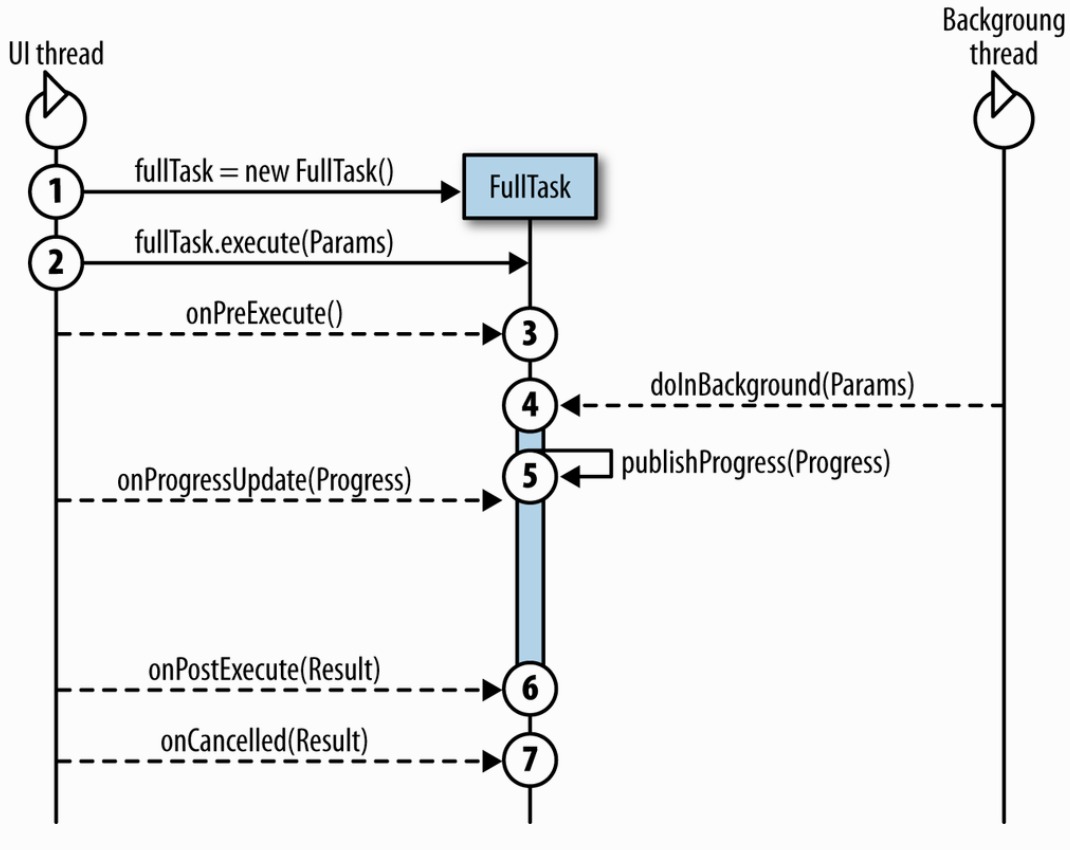
\includegraphics[width=120mm]{figures/ch7/3.png}
	\caption{The execution lifecycle of AsyncTask.}
	\label{fig7.3}
\end{figure}
The different steps are:
\begin{enumerate}
	\item Create the AsyncTask instance.
	\item Start execution of the task.
	\item First callback on the UI thread: onPreExecute. This usually prepares the UI for the long operation—e.g., by displaying a progress indicator on the screen.
	\item Callback on a background thread: doInBackground. This executes the long-running task.
	\item Report progress updates from the publishProgress method on the background thread. These trigger the onProgressUpdate callback on the UI thread, which typically handles the update by changing a progress indicator on the screen. The progress is defined by the Progress parameter.
	\item The background execution is done and is followed by running a callback on the UI thread to report the result. There are two possible callbacks: onPostExecute is called by default, but if the AsyncTask has been cancelled, the callback onCancelled gets the result instead. It is guaranteed that only one of the callbacks can occur.
\end{enumerate}
The progress update mechanism solves two use cases:
\begin{itemize}
	\item Displaying to the user how the long-running operation is progressing, by continuously reporting how many of the total tasks are executed.
	\item Delivering the result in portions, instead of delivering everything at the end in onPostExecute. For example, if the task downloads multiple images over the network, the AsyncTask does not have to wait and deliver all images to the UI thread when they are all downloaded; it can utilize publishProgress to send one image at the time to the UI thread. In that way, the user gets a continuous update of the UI.\cite{ref19}
\end{itemize}

\section{Baseline wander solutions}
In order to solve this problem, taking into account all the related problematic, we have chosen two kinds of approach. Each one will be described afterwards. The first approach will be always active, and will consist in the dynamic calculation of samples vertical axis during drawing iteration. The second is the usage of a simple moving average filter that could be activated in the app settings for the acquisition phase.

\subsection{Adaptive vertical displaying}
We decided to hold this type of solution active by default in order to maintain a solid and versatile way to overcome the worst scenario caused by a strong baseline wander. The approach works like this: at each frame drawing, we have a visible window of samples, with a length dictated from the space available on the device's screen, that we have to plot. Given that window, we know that we have to fit as many samples as we can, inside the space dedicated to that signal, the signal ECG strip. In a normal scenario, the signal will be aligned to a baseline, and so we can easy plot all the samples inside the relative strip. However in some other scenarios, it could happen that because of movement of the patient, the signal could immediately drop down. For this reason, the signal could easily go out of the available vertical space. To avoid this, we have to provide a mechanism in order to hit these cases and accordingly respond. We do this by not fixing the vertical baseline of the ECG strip, and leave it dynamic. Therefore this baseline will go up and down according to the position of the values inside the samples window. So every time, before we redraw the updated window on the screen, we compute the baseline of the signal at that moment by computing the mean of all samples. After that, we can shift the signal to plot up or down, trying to include the majority of samples on the screen. An example of the mechanism is showed in the figure \ref{fig7.4}. As you can see, starting from the second 23, a patient movement caused the baseline wander artifact, causing a drop of the D1 signal. The app by applying the dynamic displaying, it computed the new baseline of the signal, represented by the mean of all samples, and shifted all sample window accordingly. In the figure, the variation of the vertical axis is represented by $\Delta y$.\\
In this way we can overcome this type of scenario, avoiding the appliance of any kind of filtering. The latter, depending on the technique, can result in some percentage of error on the filtered ECG signal.
\begin{figure}[ht!]
	\centering
	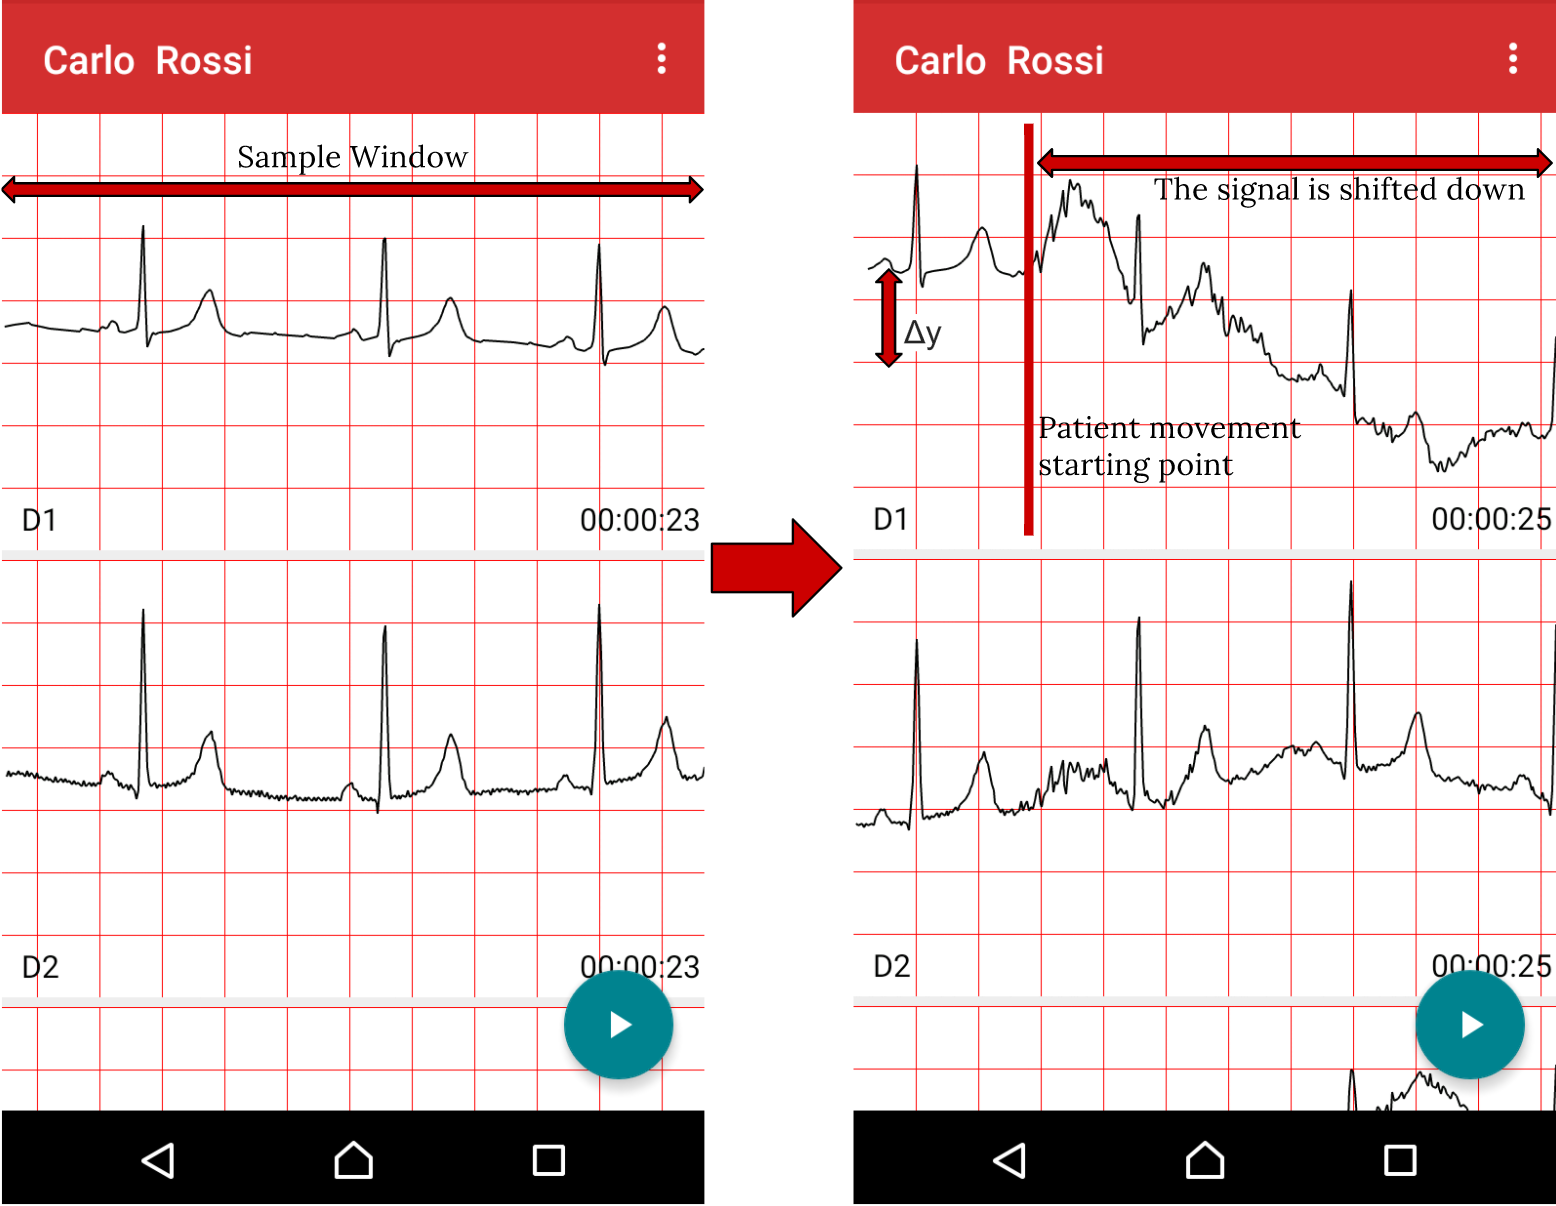
\includegraphics[width=130mm]{figures/ch7/4.png}
	\caption{The dynamic displaying result after a patient movement, causing the baseline wander artifact.}
	\label{fig7.4}
\end{figure}

\subsection{Moving average filter}
As discussed in the requirements section, many types of filtering are known to overcome to the baseline wander artifact. Some of them are capable to reduce at minimum the error on the output signal. Nevertheless this comes with a cost in computational effort, and so there is the need to mediate between the type of filtering and its related complexity.
Unfortunately in our case, putting in all the required operation, especially during real-time acquisition, where the app has to hold the bluetooth channel for transmission, interpret the transmitted signal, write to a file, derive the missing ECG lead, and plot at a reasonable rate the acquired signal, we had very limited computational availability to spend in any type of filtering in order to remove the eventual baseline wander. Therefore we decided to apply the most basic type of filtering during acquisition that is the simple moving average filtering. Given that, we are conscious about the possible distortion introduced by this filter, that's why we decided to:
\begin{itemize}
	\item Take a reasonable size for the moving average window (two seconds at least), inasmuch if it is true that as much as the window size grows, the effectiveness of the filter decreases, by doing this, we can keep the error rate low.
	\item Keep the filter deactivated by default, so that the doctor will decide when will be opportune to use it.
\end{itemize}

\section{Custom View Drawing}
Now we will talk about the most costly operation performed about our application. This was the thing on which we have spent lots of work, investigating all the problematic and different possibilities that we had in order to make the best possible implementation choice. We have mentioned earlier the computational effort that needs to be spent on signal drawing and for this reason we tried all the possible ways in order to discard the bad implementation, always having performance in our mind.

\subsection{Custom Libraries}
This was our first trial: we tried to find some libraries that could have permitted us to avoid an implementation from scratch of our drawing classes. For sure this possibility was the easiest possible. Given that our signal was not so different from other types of signals, as could be interpreted as a generic function plotted on a two dimensional system, we had quite sure that we could have found a nice plotting library and avoid useless implementation. Actually, we were able to find some well-realized libraries for handling plottings, but all of them clashed with one characteristic that we was seeking for: the customization of the rendered views, as we have said previously, has to mimic as much as possible the ECG paper on the look and also respect the required standard sizing of the same. Therefore, for this reason, we needed to discard this solution, given that some libraries permitted us to have very good displaying performance.

\subsection{Hardware Accelerated Drawing (GPU)}
Another solution, and potentially the best one, was to exploit the graphic hardware acceleration. Android is possible by using OpenGL ES, a subset of the OpenGL API designed for embedded system. The use of OpenGL can move all the graphics computations to the GPU, and so freeing up precious computing resources on the CPU. But unfortunately, in Android the usage of these libraries is not so integrated: they are written in hardware native code, which is C. This characteristic, while could of course guarantee the best performance\cite{ref20}, introduce a misalignment with the language used for developing Android application, which is Java. As a result, it is a common belief that the usage of OpenGL ES in Android is quite painful, forcing many developers to switch to better alternative libraries and frameworks, like Unity, LibGDX, Cocos2D or others. Putting aside all the problematic related to its implementation's effort, we decided to try OpenGL ES for the drawing part. With much surprise, this led us to an unexpected result: the results in performances were quite beneath the performance achieved using the CPU also for the application drawing. This relies on the fact that, as said earlier, the OpenGL libraries on Android are not so integrated, and developer are required to represent datatypes of the C language in the Java language. This may not seem problematic, but in a situation where all ECG samples need to be represented as classes, holding their coordinates in the ECG paper space in a corresponding matrix, and at each draw update there is the need to reallocate all the samples matrix, causing a remapping to the C data types, the performance improvements  are quickly drop out. For this reason, we realized that our best chance was to relying on the CPU also for the drawing, and trying as much as possible to optimize the algorithms in order to achieve the best performances.

\subsection{Not hardware Accelerated Drawing (CPU)}
Having underlined the downsides of the previous solution, we decided to spend all our energies to implement the best possible drawing code, relying on the mechanisms provided by Android for drawing operations using the CPU. This is possible using Canvas.\\
Android Canvas provides the developer with the ability to create and modify 2D images and shapes. Moreover, the Canvas can be used to create and render our own 2D objects as this class provides various drawing methods to do so. Canvas can also be used to create some basic animations such as frame-by-frame animations or to create certain Drawable objects such as buttons with textures and shapes such as circles, ovals, squares, polygons, and lines.\cite{ref21}\\
As we mentioned in the chapter about Android concurrency exploitation, all applications run on a single thread in Android. All instructions run in a sequence on the UI thread, meaning that the second instruction will not start unless the first one is finished. The UI thread as it is responsible for drawing all the objects or views on the screen and processing all events, such as screen touches and button clicks. Now the problem is that, if we have two operations scheduled to run in the same default thread or UI thread and the first operation takes too long to finish, the system will ask the user to forcibly close the application or wait for the process to complete. This scenario is called ANR (Application Not Responding).\\
Given that we wanted also to provide scrolling of the different ECG leads in our app, we could not hold this computational effort on the UI thread, which as result of drawing operations, would be blocked. Therefore we decided to assign all the drawing operations on different threads created ad-hoc. The number of threads dedicated to drawing will be decided at run time by the application, depending on the device availability, and thus allowing device scalability.\\
The use of Canvas permitted us to achieve both reasonable performances, after a deep code optimization, and high customization of the rendered view.